\section{解析延拓}
\sourcepage{44}
下面研究由函数芽的解析延拓产生的黎曼曲面的构造。
\entry{7.1}{定义}
设$X$为黎曼曲面，$u:[0,1]\to X$为曲线，$a:=u(0)$、$b:=u(1)$。若存在函数芽族$\varphi_t\in\OO_{u(t)}$（$t\in[0,1]$），满足$\varphi_0=\varphi$、$\varphi_1=\psi$，并且对每个$\tau\in[0,1]$，存在$\tau$的邻域$T\subset[0,1]$、开集$U\subset X$及函数$f\in\OO(U)$，使$u(T)\subset U$且对所有$t\in T$有$\rho_{u(t)}(f)=\varphi_t$，则称全纯函数芽$\psi\in\OO_b$由$\varphi\in\OO_a$沿曲线$u$\textbf{解析延拓}（analytic continuation）得到。

由$[0,1]$紧，此条件等价于（见图5）：存在分割$0=t_0<t_1<\cdots<t_n=1$、区域$U_i\subset X$及全纯函数$f_i\in\OO(U_i)$，使$u([t_{i-1},t_i])\subset U_i$，且：
(i)$\varphi$为$f_1$在$a$处的芽，$\psi$为$f_n$在$b$处的芽；
(ii)$f_i|_{V_i}=f_{i+1}|_{V_i}$（$i=1,\ldots,n-1$），其中$V_i$为$U_i\cap U_{i+1}$中包含$u(t_i)$的连通分支。
\sourcepage{45}
\begin{center}\begin{minipage}{\linewidth}\centering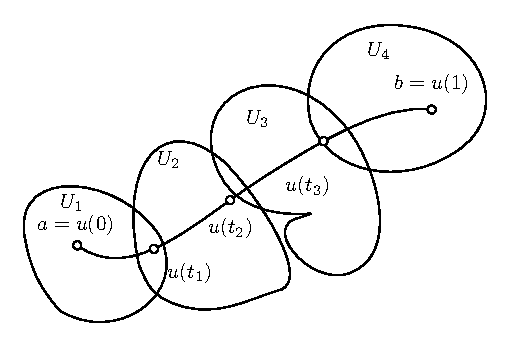
\includegraphics[width=.65\textwidth]{figures/fig05-tikz.pdf}\\图5\end{minipage}\end{center}
对全纯函数层$\OO$作(6.7)的构造，得到$p:|\OO|\to X$。下一引理说明，可借此映射解释沿曲线的解析延拓。
\entry{7.2}{引理}
设$X$为黎曼曲面，$u:[0,1]\to X$从$a$到$b$。则$\psi\in\OO_b$是$\varphi\in\OO_a$沿$u$的解析延拓，当且仅当存在曲线$u$的提升$\widetilde u:[0,1]\to|\OO|$使$\widetilde u(0)=\varphi$、$\widetilde u(1)=\psi$。
\begin{proof}
(a) 若$\psi$为所述延拓，取(7.1)的芽族$\varphi_t$。由$|\OO|$的拓扑定义，$t\mapsto\varphi_t$为连续映射，因而是满足端点条件的提升。

(b) 反之，若存在这样的提升，令$\varphi_t:=\widetilde u(t)$，则$\varphi_t\in\OO_{u(t)}$且端点正确。给定$\tau$，选$\widetilde u(\tau)$的开邻域$[U,f]$。存在$\tau$的邻域$T$使$\widetilde u(T)\subset[U,f]$，故$u(T)\subset U$且$\varphi_t=\rho_{u(t)}(f)$（$t\in T$）。这正是解析延拓的条件。
\end{proof}
由提升唯一性(4.8)，函数芽的解析延拓若存在，就唯一确定。另一个推论是单值性定理。
\entry{7.3}{单值性定理}
设$X$为黎曼曲面，$u_0,u_1:[0,1]\to X$为从$a$到$b$的同伦曲线。设$u_s$（$0\le s\le1$）为从$u_0$到$u_1$的形变，函数芽$\varphi\in\OO_a$可沿每条$u_s$解析延拓。
\sourcepage{46}
则沿$u_0,u_1$所得的函数芽$\psi\in\OO_b$相同。
\begin{proof}
对局部同胚$|\OO|\to X$应用(4.10)；由(6.10)，$|\OO|$为Hausdorff空间。
\end{proof}
\entry{7.4}{推论}
设$X$为单连通黎曼曲面，$a\in X$，$\varphi\in\OO_a$可沿从$a$出发的每条曲线解析延拓。则存在整体定义的全纯函数$f\in\OO(X)$使$\rho_a(f)=\varphi$。

\textbf{注记。}由恒等定理，$f$唯一。
\begin{proof}
对$x\in X$，令$\psi_x\in\OO_x$为$\varphi$沿任一从$a$到$x$的曲线延拓所得芽。由$X$单连通，它不依赖曲线选择。令$f(x):=\psi_x(x)$，则$f$在$X$上全纯且$\rho_a(f)=\varphi$。
\end{proof}
\entry{7.5}{}
一般地，即使函数芽能沿起终点相同的两条曲线延拓，所得终点芽也可能不同。因此，把从给定芽经解析延拓得到的所有芽合在一起，就得到多值函数。下面将精确说明这一情形。

设$X,Y$为黎曼曲面，$\OO_X,\OO_Y$为其全纯函数层，$p:Y\to X$无分歧全纯。由$p$局部双全纯，对每个$y\in Y$诱导同构$p^*:\OO_{X,p(y)}\to\OO_{Y,y}$。以$p_*:\OO_{Y,y}\to\OO_{X,p(y)}$表示其逆。
\entry{7.6}{定义}
设$X$为黎曼曲面，$a\in X$、$\varphi\in\OO_a$。称四元组$(Y,p,f,b)$为$\varphi$的一个\textbf{解析延拓}，如果：
(i)$Y$为黎曼曲面，$p:Y\to X$无分歧全纯；
(ii)$f$为$Y$上的全纯函数；
(iii)$b\in Y$满足$p(b)=a$且$p_*(\rho_b(f))=\varphi$。

若还满足下述泛性质，则称此延拓\textbf{极大}：对$\varphi$的任意其他解析延拓$(Z,q,g,c)$，存在保纤维全纯映射$F:Z\to Y$，使$F(c)=b$且$F^*(f)=g$。
\sourcepage{47}
极大解析延拓在同构意义下唯一。事实上，若$(Y,p,f,b)$、$(Z,q,g,c)$均极大，则还存在保纤维全纯映射$G:Y\to Z$使$G(b)=c$、$G^*(g)=f$。复合$F\circ G$保纤维且固定$b$，由(4.8)等于$\mathrm{id}_Y$。同理$G\circ F=\mathrm{id}_Z$，故$G$双全纯。
\entry{7.7}{引理}
设$(Y,p,f,b)$为$\varphi\in\OO_a$的解析延拓，$v:[0,1]\to Y$从$b$到$y$。则芽$\psi:=p_*(\rho_y(f))\in\OO_{p(y)}$为$\varphi$沿$u:=p\circ v$的解析延拓。
\begin{proof}
令$\varphi_t:=p_*(\rho_{v(t)}(f))\in\OO_{u(t)}$，则$\varphi_0=\varphi$、$\varphi_1=\psi$。给定$t_0$，选$v(t_0)$、$u(t_0)$的开邻域$V,U$使$p|_V:V\to U$双全纯。令$q:U\to V$为逆，$g:=q^*(f|_V)$。则对每个$\eta\in V$，$p_*(\rho_\eta(f))=\rho_{p(\eta)}(g)$。存在$t_0$的邻域$T$使$v(T)\subset V$，故对$t\in T$，$\rho_{u(t)}(g)=p_*(\rho_{v(t)}(f))=\varphi_t$。这证明所述延拓关系。
\end{proof}
\entry{7.8}{定理}
设$X$为黎曼曲面，$a\in X$，$\varphi\in\OO_a$为全纯函数芽。则$\varphi$存在极大解析延拓$(Y,p,f,b)$。
\begin{proof}
令$Y$为$|\OO|$中包含$\varphi$的连通分支，仍以$p$表示$|\OO|\to X$在$Y$上的限制。由(4.6)，局部同胚$p:Y\to X$使$Y$自然成为黎曼曲面，且$p$全纯。每个$\eta\in Y$为$p(\eta)$处的函数芽，定义$f(\eta):=\eta(p(\eta))$。容易看出$f$全纯，且对每个$\eta\in Y$有$p_*(\rho_\eta(f))=\eta$。令$b:=\varphi$，便得一个解析延拓。

为证极大性，取任一其他延拓$(Z,q,g,c)$。对$\zeta\in Z$，令$x:=q(\zeta)$。由(7.7)，芽$q_*(\rho_\zeta(g))\in\OO_x$由$\varphi$沿从$a$到$x$的曲线延拓得到。由(7.2)，$Y$恰由所有如此得到的芽组成。因此存在唯一$\eta\in Y$满足$\eta=q_*(\rho_\zeta(g))$，定义$F(\zeta):=\eta$。容易验证$F$为保纤维全纯映射，$F(c)=b$且$F^*(f)=g$。
\end{proof}
\sourcepage{48}
\textbf{注记。}本节用于全纯函数芽的方法同样可处理亚纯函数芽，只须考虑映射$|\MM|\to X$。目前尚未处理分歧点；下一节将对代数函数这一特殊情形讨论它们。
\subsection*{习题（第7节）}
\entry{7.1}{}
设$p:Y\to X$为黎曼曲面之间的无分歧全纯覆盖，$f:Y\to\C$全纯。令$b\in Y$、$a:=p(b)$、$\varphi:=p_*(\rho_b(f))\in\OO_a$。证明$(Y,p,f,b)$为$\varphi$的极大解析延拓，当且仅当：对任意不同的$b_1,b_2\in p^{-1}(a)$，芽$\varphi_1:=p_*(\rho_{b_1}(f))$、$\varphi_2:=p_*(\rho_{b_2}(f))$不同。
\entry{7.2}{}
设$\varphi\in\OO_a$可沿黎曼曲面$X$中每条从$a$出发的曲线解析延拓，$(Y,p,f,b)$为其极大解析延拓。证明$p:Y\to X$为覆盖映射。
